\documentclass[a4paper,12pt,report]{jsbook}
%ページに綴じ代をつくる
\setlength{\textwidth}{38zw}
\setlength{\oddsidemargin}{0.5cm}
%小島先輩との変更点は下の定義とページ下のBibtex
\def\BibTeX{{\rmfamily B\kern-.05em{\scshape i\kern-.025em b}\kern-.08em
 T\kern-.1667em\lower.7ex\hbox{E}\kern-.125em X}}
 %共通設定
\renewcommand{\bibname}{参考文献}
\renewcommand{\theenumi}{\roman{enumi}}
\usepackage{makeidx}
\pagestyle{headings}
\pagenumbering{roman}
\usepackage{graphicx}
\usepackage[fleqn]{amsmath}
\usepackage{amsthm}
%\usepackage{amssymb}
\usepackage{latexsym}
\usepackage{newtxtext}
\usepackage{url}
\usepackage{here}
\usepackage{float}
\usepackage[varg]{newtxmath}
\usepackage{enumitem}
\usepackage{multirow}
\usepackage{bm}
\usepackage{amsmath}
\usepackage{color}
\usepackage{diagbox}
\usepackage{booktabs}
\usepackage{bicaption}
% 2つ目のキャプションを「Fig.」に設定
\captionsetup[figure][bi-second]{name=Fig.}
\captionsetup[table][bi-second]{name=Tab.}
%\usepackage[dvipdfmx]{hyperref}
\newcommand{\argmax}{\mathop{\rm argmax}\limits}
\newcommand{\argmin}{\mathop{\rm argmin}\limits}
\makeindex
\begin{document}
%
% 表紙
%
\begin{titlepage}
\begin{center}
{\large 令和6年度卒業論文\\}
\vspace{2.5cm}
{\HUGE ビデオビットレート制御関数を用いた他ユーザ使用帯域制限の抑制\\}
{\huge Suppression of Bandwidth Limitation for Other Users Using Video Bitrate Control Function\\}
\vspace{3cm}
{\Large
  芝浦工業大学 工学部 情報通信工学科\\
  \vspace{3mm}AF21014 菊地 悠李\\
  \vspace{2cm}上岡研究室\\
}%各所にあるvspaceの値を調整して1ページに収まるようにしましょう.
\end{center}
\end{titlepage}
\tableofcontents
\listoffigures%図のリストを作る
\listoftables%表のリストを作る(表を全く使わない場合には,この行は削除)
\newpage
\newpage
\pagenumbering{arabic}
\setcounter{page}{1}
%%%%%%%%%%%%%%%%%%%%%%%ここから本文を書きましょう%%%%%%%%%%%%%%%
%各章毎にファイルを分割して\inputで読み込ませると管理が楽
\chapter{序論}
近年,ストリーミングサービスの普及と需要の増加に伴い,ネットワークトラヒックが増加し,インターネットトラヒックの中で動画が大きな割合を占めている.このトラヒックの増加により,安定して高画質な動画を配信することが重要な課題となっている\cite{kison}\cite{motomoto}.このような課題に対して,サーバとユーザ間で動画データを適応的に送信する技術として,アダプティブビットレートストリーミング(ABS)が活用されている.しかし,動画に関するトラヒックが大きく占め,限られているネットワーク帯域幅は,ユーザ数や通信量の変動,無線通信環境の特性,TCPの輻輳制御などの要因によって動的に変化する\cite{C.Wang}.このような課題は,ABSにおいて,ユーザの利己的な行動が帯域幅の利用効率低下や,ユーザ間の不公平なリソース配分によるユーザの動画再生中断につながり,対処しきれない\cite{kison}\cite{C.Wang}.この問題を解決するために,ユーザのビデオビットレートを制御し,安定して高画質な動画配信を実現するビデオビットレート制御の研究が進められている\cite{kison}\cite{motomoto}\cite{Thang}\cite{Mao}\cite{Xu}.

特に,複数のユーザが共有するリンクがボトルネックとなる場合,リンクの帯域幅が逼迫し,あるユーザの要求するビデオビットレートが他のユーザの使用帯域幅に影響を与える.結果として,共有しているユーザは希望するビデオビットレートのデータが十分に送信されない,あるいは動画の再生が停止することがある.このような課題を解決するためには,ユーザ間の相互影響を考慮した適切なビデオビットレート制御が必要である.
また,近年,ビデオコンテンツの品質に対するユーザ満足度を表す体験の質(QoE)に焦点を当てた方法が,サービスプロバイダーおよびネットワークプロバイダーの注目を集めている\cite{kison}.特に,HTTPモバイルストリーミングにおけるQoE評価手法に関する研究では,ユーザの行動パターンや動画視聴環境がQoEに与える影響が示されている\cite{Y.Huang}.同研究では,QoEの主な要因として,視聴動画の流暢性,つまり動画の再生停止が大きな影響を与えることが指摘されている.このため,動画の再生停止の原因であるバッファの枯渇の起きない適応的なビットレート制御が求められる.

本研究では,ユーザのビデオビットレートが他のユーザの帯域使用に及ぼす相互依存関係を,ゲーム理論を用いてモデル化する.ゲーム理論は,複数のユーザが共有資源を取り合う際に生じる相互依存関係を数理モデルを通じて解析する理論である\cite{okada2011}.本研究では,このゲーム理論を基盤に,ユーザの戦略となる要求ビデオビットレートに応じてユーザ毎に異なるペナルティを導入し,ユーザの要求ビデオビットレートが他ユーザの帯域使用に及ぼす影響を考慮した新たな利得関数を提案する.この提案利得関数を用いることにより,低ビットレートユーザに過渡な制限を与えず,各ユーザのビデオビットレート要求に応じた帯域割り当ての実現可能性を示す.さらに,この提案手法では既存研究\cite{kison}のビデオビットレート制御に比べ,バッファの貯蓄量が多く,動画の再生停止が起きにくいことを示す.

本論文の構成は以下の通りである.2章にて関連研究とその問題点について述べ,3章3,4節にて既存研究におけるゲーム理論を用いたレート制御法の説明を行う.3章5節にて提案するレート制御手法を説明をし,4章にて数値解析とその結果を述べる.5章にてまとめと本研究における問題点を述べる.


%%リンク共有時の動画再生停止を防ぐための既存の画質レート制御関数では,自身の要求画質による他ユーザの転送レートへの影響が考慮されていない.そこで本研究では,このような他ユーザの転送レートへの影響を考慮した画質レート制御関数を提案する.

\chapter{関連研究}

これまでに数多くのビデオビットレート制御に関する研究が行われてきた.

帯域幅推定に着目したビデオビットレート制御の研究がある.
Thangら\cite{Thang}は,短期的な帯域幅変動に対応し,ビットレートを安定させるため,ユーザの使用帯域推定に基づく適応的リクエスト方法を提案した.この手法では,スムージング係数の調整により短期的な変動に安定して対応しつつ,大きな変化には迅速に適応可能とした.また,メタデータに品質情報を加えることで,最適な選択を行い高品質なストリーミングを安定して提供できるようにしている.
また,実際のアプリケーションでは,ユーザの使用帯域や帯域幅を正確に推定することは容易ではない.

そこで,Maoら\cite{Mao}は,ユーザの使用帯域を正確に推定することに基づいた深層強化学習レート適応アルゴリズムを提案した.ニューラルネットワークを利用して,過去のデータからビットレート選択を自動で学習し,適応することで高いQoEを実現した.しかし,大量のデータが必要である点や,様々なビデオの特性やネットワーク条件において,同様に適応できるか等の課題がある.

さらに,ユーザの体感品質であるQoEを向上させるため,QoE最大化に基づく動的ビデオビットレート制御方法が研究された.
Xuら\cite{Xu}は,ユーザのQoEをビットレート,再生バッファの飢餓確率,および連続再生時間を組み合わせたモデルで評価し,ユーザの使用帯域変動とバッファ長に基づいてビットレートを動的に調整する2つのビデオビットレート制御アルゴリズムを提案し,ストリーミングの効率と安定性を考慮し,ユーザのQoEを最大化した.
しかし,このような手法ではユーザ個人ごとに制御を行っているため,原因となっているユーザ間の相互影響を考慮できていない.

Yanagisawa\cite{kison}やYuanら\cite{motomoto}は,複数のユーザがリンクを共有する状況をゲーム理論を用いて考慮したビデオビットレート制御手法を提案している.これらの手法は,共有リンクの帯域幅を共有資源として複数のユーザが帯域を取り合う状況をゲーム理論でモデル化し,利得関数を用いてユーザ毎に最適なビデオビットレートを決定している.
しかし,各ユーザのビデオビットレートが他ユーザの帯域への影響を十分に反映できていない.

本研究では,既存手法\cite{kison}と\cite{motomoto}におけるゲーム理論を用いたレート制御手法において,複数ユーザ間の相互影響を考慮した制御関数に改善する.
\chapter{提案法}
\section{想定システム}
本稿では,図\ref{fig:soutei}に示すような複数ユーザが利用するリンクに対してボトルネックリンクが存在する環境を仮定する.
\begin{figure}[hh]
\centering
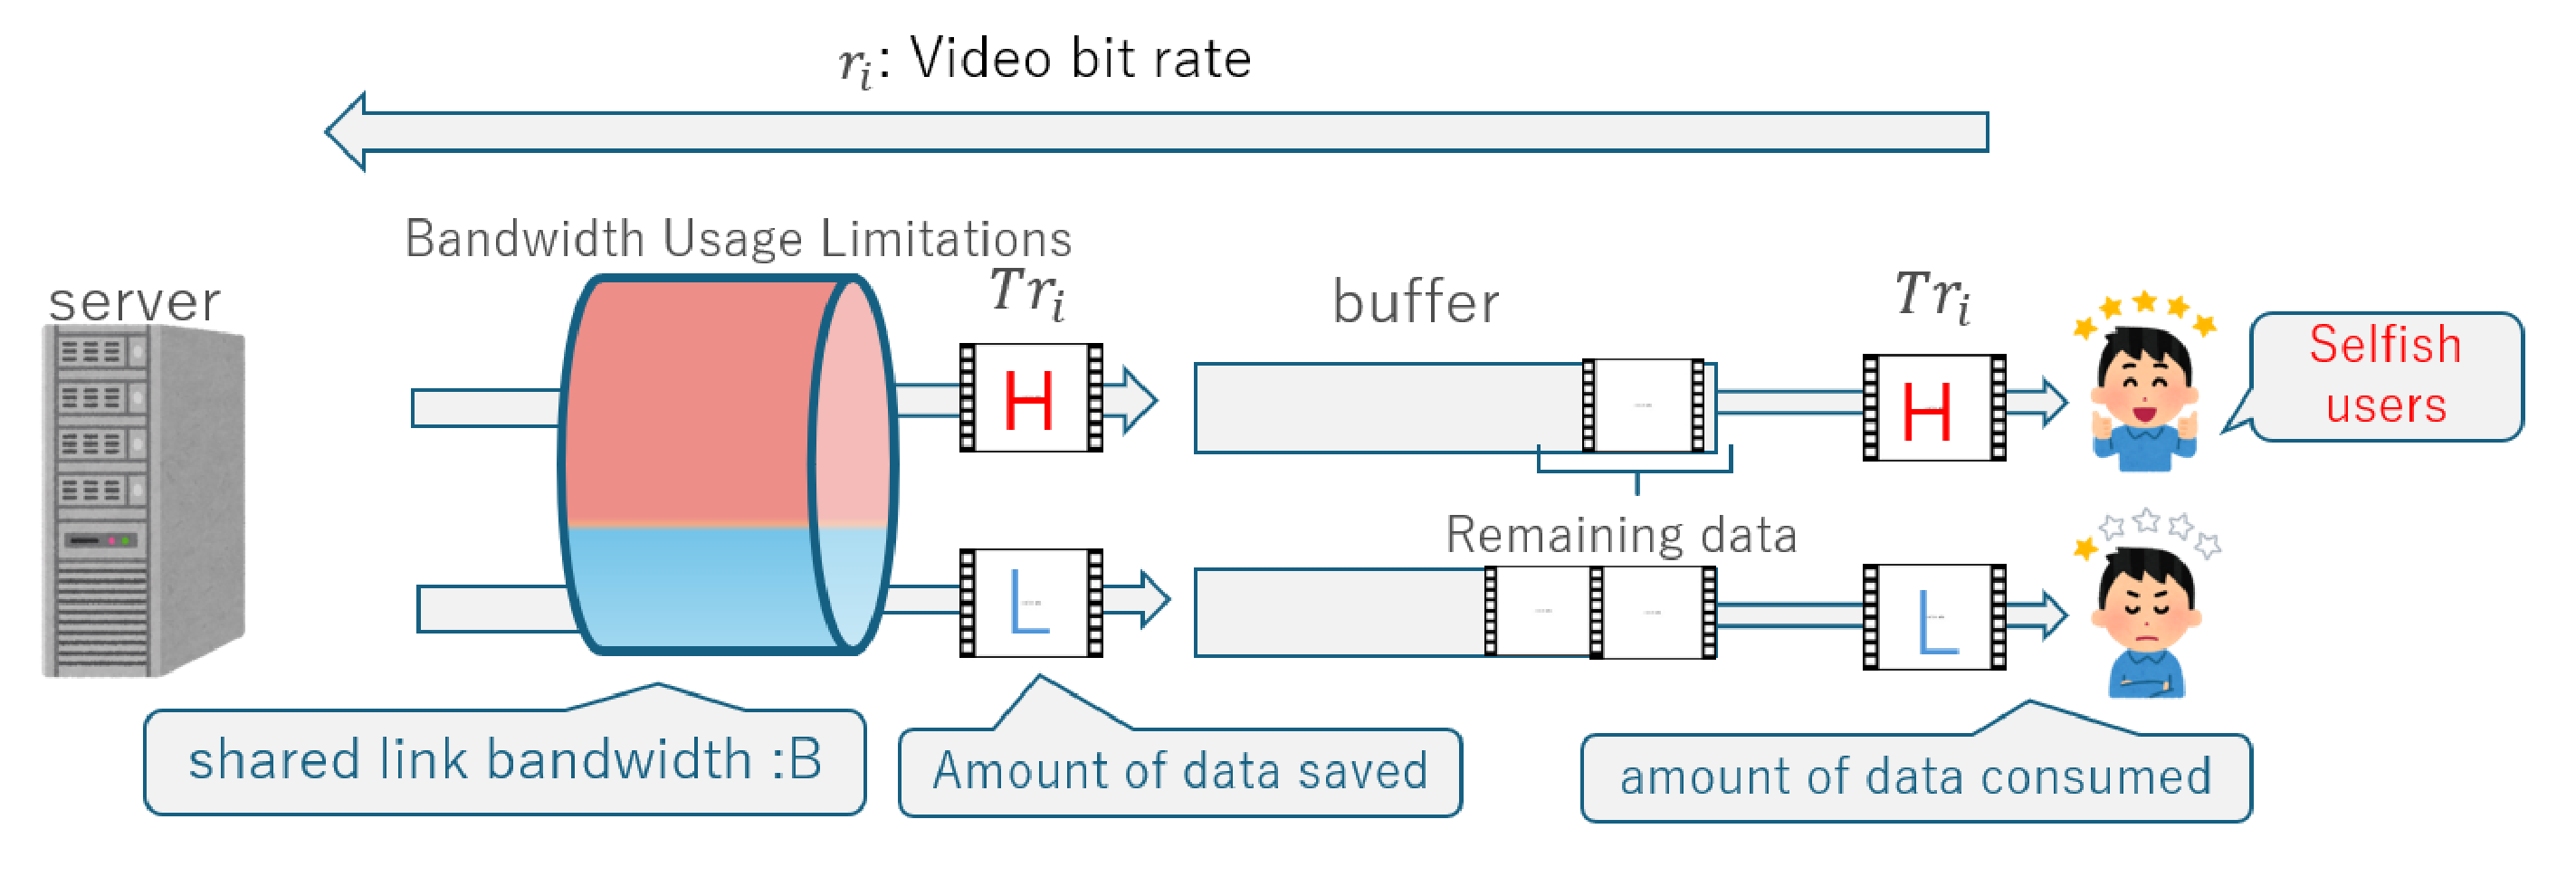
\includegraphics[scale=0.3]{sisutemu.eps}
\bicaption{想定システム}%
            {Assumed system}
\label{fig:soutei}
\end{figure}
ボトルネックリンクの環境では,使用可能帯域幅が狭まっており,ユーザの要求ビデオビットレートが共有しているその他ユーザの使用するはずの帯域に大きく影響し,使用可能帯域を狭め,影響を受けたユーザが動画の再生停止に陥りやすくなる問題がある.そこで,本研究では各ユーザの要求ビデオビットレートによるその他ユーザの使用帯域への影響を考慮するために,ゲーム理論を用いてこの問題をモデル化する.

\section{提案法}
処理の流れは,図\ref{fig:syori}に示す\cite{motomoto}.
まず初めに,ユーザはサーバにセグメント単位で,動画のビデオビットレートを要求する.次に,サーバ側で要求されたビデオビットレートと利用帯域幅の大きさを考慮して,提案利得関数を用いてナッシュ均衡点となる最適ビデオビットレートを導出する.その後,サーバ側で決定したビデオビットレートのデータをユーザ側に送信する流れである.本研究では,この流れの利得関数の改善に着目して提案を行う.

\begin{figure}[hh]
\centering
\includegraphics[scale=0.23]{syori.eps}
\bicaption{処理の流れ}%
            {Processing flow}
    \label{fig:syori}
\end{figure}

ゲーム理論では,相手のとる戦略を考慮しながら自身の利益が最大となる戦略をとる数理モデルを解析する.ストリーミングにおける帯域分配問題において,ユーザ同士は意思疎通を図り協力することができないため,そのようなユーザが協力できない状況をモデル化する,非協力ゲームを用いる.非協力ゲーム理論を用いることで,複数の利己的なユーザが,帯域幅を争う状況ををモデル化し,複数ユーザ間の相互影響における動画の再生停止に陥りやすくなる問題を解析する.

本研究では,ユーザ$i$の最適ビデオビットレート$r_i^*$を決定するため,非協力ゲームを用いて,各ユーザが自身の戦略であるビデオビットレートを変更してもこれ以上利益が増えない状態である最適応答となる戦略レートの組み合わせ(以降,ナッシュ均衡点と呼ぶ)を求める.本研究では,$N=$\{$1,2,3,\dots,n$\},ユーザの選択可能レート$r_i$,ユーザ$i$の利得関数を$f_i$とすると,$G=\left(N,{r_i}_{(i\in N)},{f_i}_{(i\in N)}\right)$とモデル化することができる.
本研究では,ナッシュ均衡点を利得関数によって決定する.

\section{ビデオビットレート制御法}

%%下の説明をどこに入れるか
本研究では,既存研究\cite{kison}と\cite{motomoto}で用いられている利得関数を基に,関数の一部を変更したものであるため,まずは既存研究での利得関数\cite{kison}\cite{motomoto}について説明を行う.

以下に非協力ゲームレート制御法\cite{kison}の$f_i$を示す.
\begin{equation}
 f_{i}=\underbrace{q_{i}(r_{i,k})}_{(\rm{A})}+\underbrace{\mu\Delta{b^{\rm{est}}_{i,k}}(r_{i,k},\mathbf{r}_{-i,k})}_{(\rm{B})}+\underbrace{\gamma_i{R}_{\rm{f}}(r_{i,k})}_{(\rm{C})}.
 \label{eq:f1}
\end{equation}
以下に,より詳細な式を示す.
\begin{equation}
\begin{split}
  f_i(r_k) = &\ \underbrace{\alpha_{\text{ct}} \log(1 + |\beta_{\text{ct}}| r_{i,k})}_{(\rm{A})} \\
  &+ \underbrace{\mu \frac{2 e^{p(b_{i,k-1} - b_s)}}{1 + e^{p(b_{i,k-1} - b_s)}}\left(  T r_{i,k} \right) - \mu \omega  \left( T \frac{r_{i,k}^2 + r_{i,k} \sum_{l \neq i} r_{l,k}}{B_W} \right)}_{(\rm{B})} \\
  &+ \underbrace{\gamma_i \left( -m(r_{i,k} - r_{i,k-1} + r^{(J)})^2 - 2m(r_{i,k} - r_{i,k-1}) \right)}_{(\rm{C})}
  \label{eq:syousai}
\end{split}
\end{equation}



非協力ゲームレート制御法\cite{kison}では,式\eqref{eq:f1}基い\eqref{eq:syousai}を用いて最適レートを導出していた.
(A)項はビデオビットレートのみから得られる嬉しさを表す単調増加の関数である.
(B)項はバッファの変動量を用いてユーザのビデオビットレートを制御する関数である.
(C)項は前のセグメントで決定したビデオビットレートとの変動差を抑える関数である.
ここで,大きくビデオビットレートの制御を行っているのは,(B)項であった.
次に,(B)項を説明する.以下に,(B)項の基本構造を示す.
\begin{equation}
 f_{buffer}=Tr_{i,k}-Tr_{i,k}\underbrace{(\frac{\sum^N_{i=1}r_{i,k}}{B})}_{\rm{(D)}}
 \label{eq:f_{buffer}}
\end{equation}

式\eqref{eq:f_{buffer}}は,あるセグメントにおけるバッファの変動量を表している.
$T$はセグメント長[s],$r_i$はビデオビットレート[Mbps],$B$はリンクの全帯域幅[Mbps]を表す.
1項目はバッファにたまるのデータ量を表し,2項目は1項目のデータがバッファに溜まりきるまでの時間でバッファから消費されるデータ量を表す.

ここで,式\eqref{eq:f_{buffer}}の(D)は要求に対するペナルティを与える補正項を表している.全帯域に対して全ユーザの合計要求ビデオビットレートの方が大きいと,要求ビデオビットレートのデータがバッファにダウンロードされるまでに時間がかかり,その間,よりバッファからデータが消費される.バッファにデータがたまっていない状態をバッファ枯渇と言い,再生できる動画データがないため,動画の再生停止が起きる.

この補正項では,ユーザ毎の要求ビデオビットレートの大きさに応じてペナルティを与えていない.そのため,帯域を狭めている大きいビデオビットレートを要求した利己的なユーザも,小さいビデオビットレートを要求したユーザも同じペナルティが与えられ,制限がかけられる.それは,以下の表\ref{tb:ritoku1}を見れば明らかである.表\ref{tb:ritoku1}では,セグメント長が1sで二人のユーザが4Mbpsの帯域を争ったときの二人の利得を示す.二人のユーザは$1\sim6$Mbpsのビットレートを要求することができ,各レートを要求したときの利得を式\eqref{eq:f_{buffer}}を用いて計算している.表内の値は,(ユーザ1の利得,ユーザ2の利得)である.
%%以下101行目の1文修正箇所

\begin{table}[h]
    \centering
    \bicaption{非協力ゲームレート制御法\cite{motomoto}の利得表}
            {Non-cooperative game rate control method\cite{motomoto} gain table}
    \scalebox{0.7}{
    \begin{tabular}{|c|c|c|c|c|c|c|}
        \hline
        \diagbox{user1}{user2} & 1 & 2 & 3 & 4 & 5 & 6 \\ \hline
        1 & (0.5, 0.5) & (0.25, 0.5) & (0.0, 0.0) & (-0.25, -1.0) & (-0.5, -2.5) & (-0.75, -4.5) \\ \hline
        2 & (0.5, 0.25) & (0.0, 0.0) & (-0.5, -0.75) & (-1.0, -2.0) & (-1.5, -3.75) & (-2.0, -6.0) \\ \hline
        3 & (0.0, 0.0) & (-0.75, -0.5) & (-1.5, -1.0) & (-2.25, -3.0) & (-3.0, -5.0) & (-3.75, -7.5) \\ \hline
        4 & (-1.0, -0.25) & (-2.0, -1.0) & (-3.0, -2.25) & (-4.0, -4.0) & (-5.0, -6.25) & (-6.0, -9.0) \\ \hline
        5 & (-2.5, -0.5) & (-3.75, -1.5) & (-5.0, -3.0) & (-6.25, -5.0) & (-7.5, -7.5) & (-8.75, -10.5) \\ \hline
        6 & (-4.5, -0.75) & (-6.0, -2.0) & (-7.5, -3.75) & (-9.0, -6.0) & (-10.5, -8.75) & (-12.0, -12.0) \\ \hline
    \end{tabular}
    }
    \label{tb:ritoku1}
\end{table}

縦軸のユーザ1のみが6Mbps,横軸のユーザ2が1Mbpsをとった時のそれぞれの利得は,利己的な要求をしているユーザ1のみだけでなく,低ビデオビットレートを要求しているユーザ2にもペナルティがかかり,ユーザ2の利得も同時に下がっている.

そのため,本研究ではユーザの要求ビデオビットレートと他ユーザへの影響度合いを考慮したペナルティ関数に変更する.


\section{提案利得関数}
次に提案する利得関数について説明する.以下にその式を示す.
\begin{equation}
    f_{\mathrm{buffer}}(i) = Tr_{i,k} - Tr_{i,k}\underbrace{\left(\frac{r_{i,k}}{B\left(1-\frac{r_{i,k}}{\sum^N_{j=1}r_{j,k}}\right)}\right)}_{\rm{E}}
    \label{eq:f_buffi}
\end{equation}

本利得関数では,ユーザ$i$のビデオビットレート要求が他ユーザの使用帯域に与える影響を評価する補正項を導入している.次に,Eの補正項の具体的な式を示す.
\begin{equation}
    f_{\mathrm{penalty}}=\frac{r_{i,k}}{B\left(1-\frac{r_{i,k}}{\sum^N_{j=1}r_{j,k}}\right)}
    \label{eq:f_{penalty}}
\end{equation}

この補正項は,ユーザ$i$の使用可能帯域の割合を
\begin{equation}
    B_{i}=B\frac{r_{i,k}}{\sum^N_{j=1}r_{j,k}}
    \label{eq:B_{i}}
\end{equation}
を用いて算出し,それに基づいて他ユーザの使用可能帯域への影響を評価するものである\cite{johari}.具体的には,全帯域$B$からユーザ$i$の使用可能帯域を引いた値が,残りの他ユーザの使用可能帯域を表している.この補正項\ref{eq:f_{penalty}}により,ユーザ$i$の利得は,自身のビデオビットレート要求が他ユーザの使用可能帯域をどの程度圧迫するかに応じて調整される.

また,$r_i$のみを増加させた場合,式\ref{eq:B_{i}}の値が増加し,補正項の分母が減少するため,ユーザ$i$のペナルティが増加する.一方,他ユーザも同時にビデオビットレートを増加させると,全帯域$B$が要求比率に基づき分配され,結果として全ユーザに均等なペナルティが与えられる.つまり,ユーザ$i$のみが利己的な要求を行った場合,そのペナルティが最も大きくなる.
\chapter{数値解析}
\section{利得の比較}
本解析では,ユーザ数$N=2$,セグメント長$T=1$[s],全帯域幅$B = 4$[Mbps] ,ユーザが選択できるビデオビットレート$r_i$は(1,2,3,4,5,6)[Mbps]とした場合を想定した.

図\ref{fig:kisonritoku}と図\ref{fig:teianritoku}は,ユーザ2のビデオビットレートを1Mbpsに固定し,ユーザ1のビデオビットレートを変化させた際の各ユーザの利得遷移を示している.
ユーザ1が高ビットレートを要求するにつれて,帯域幅に影響を与える利己的な要求をするユーザになっていることを表す.一方,ユーザ2は1Mbpsと帯域幅にあまり影響を与えないユーザとした.
図\ref{fig:kisonritoku}では非協力ゲームレート制御法の利得関数\ref{eq:f_{buffer}}から得られる利得の遷移を示す.
図\ref{fig:teianritoku}では提案する利得関数\ref{eq:f_buffi}から得られる利得の遷移を示す.

図\ref{fig:kisonritoku}より非協力ゲームレート制御法\cite{kison}\cite{motomoto}では,ユーザ1のビットレートが増加するにつれ,ユーザ2の利得が大きく減少している.つまり,帯域に影響を与えるユーザ1だけでなく,帯域に影響を与えないユーザ2にも過渡に利得減少を与えている.

一方,提案した利得関数\ref{eq:f_buffi}を用いることで,ユーザ2に対する過渡な制限を回避し,利得の減少を抑制することができた.また,同時に帯域に影響を与えるユーザ1に対して,影響を大きく与える高ビットレートになるにつれて,大きく利得減少を与えている.

これにより,提案する改良法は,各ユーザのビデオビットレートが他ユーザの使用帯域に与える影響を考慮し,特定のユーザへの過渡な利得減少を抑える帯域割り当てを可能にすると言える.

\begin{figure}[tp]
  \centering
  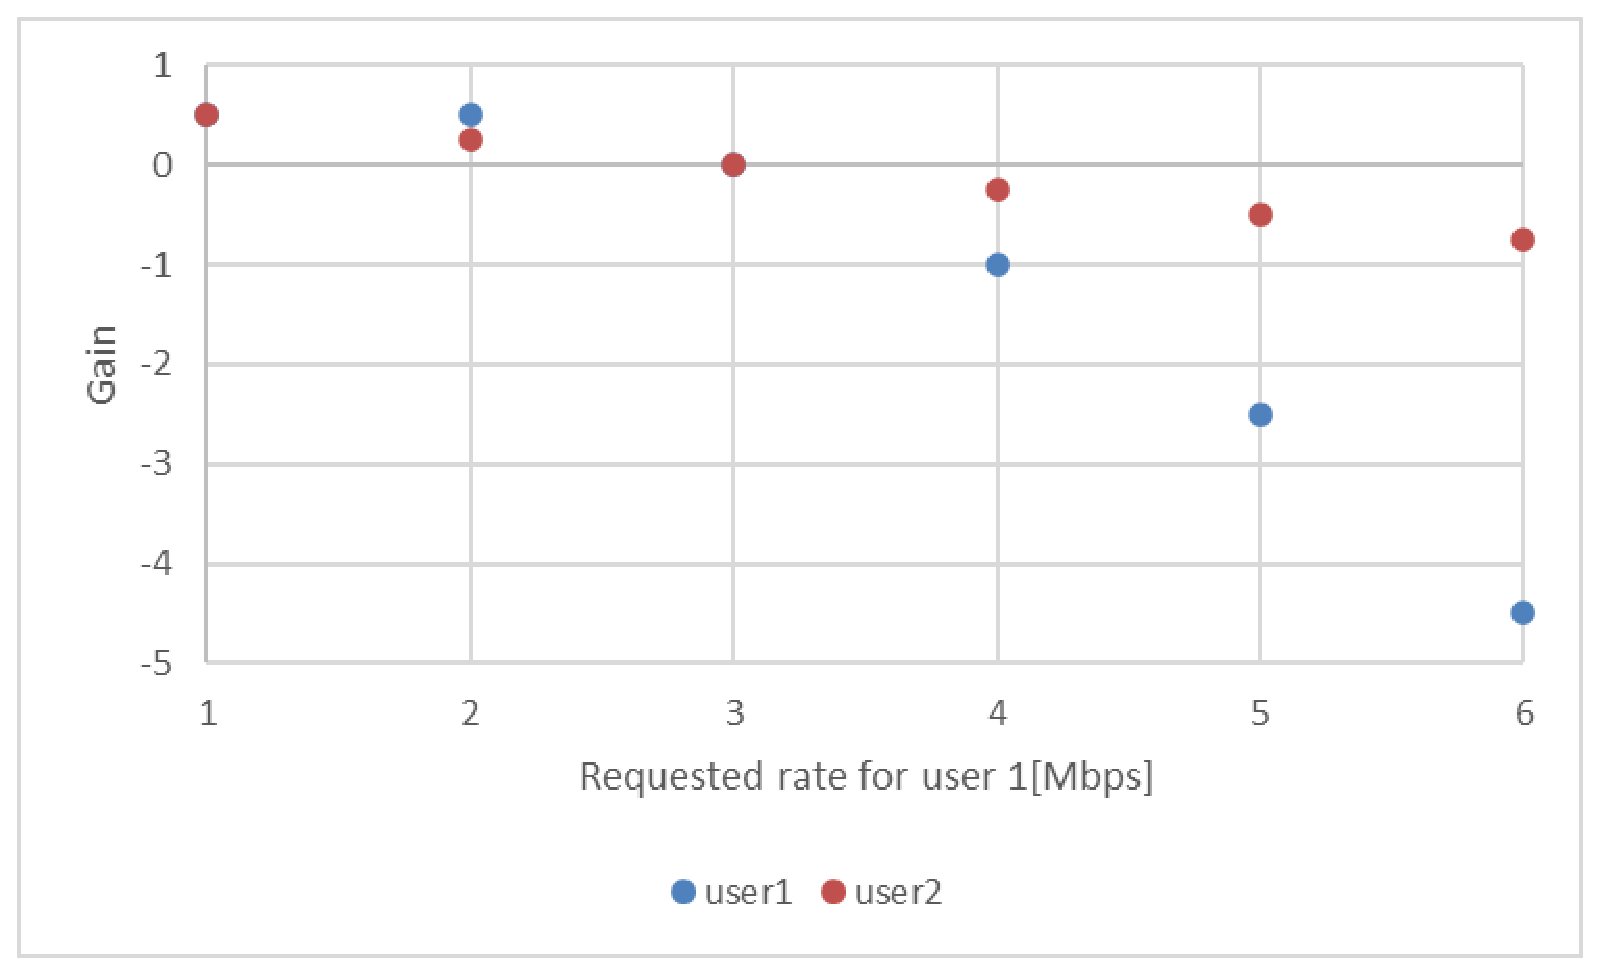
\includegraphics[scale=0.45]{kison.eps}
  \bicaption{ユーザ2が1Mbps要求時の非協力ゲームレート制御法\cite{kison}\cite{motomoto}の利得遷移}%
            {Gain transition of the non-cooperative game rate control method when user 2 requests 1 Mbps}
    \label{fig:kisonritoku}
\end{figure}

\begin{figure}[bp]
  \centering
  \includegraphics[scale=0.45]{teian.eps}
  \bicaption{ユーザ2が1Mbps要求時の提案関数の利得遷移}%
            {Gain transition of the proposed function when user 2 requests 1 Mbps}
    \label{fig:teianritoku}
\end{figure}


\section{貯蓄バッファ量の比較}

本解析では,4人のユーザが全帯域幅$B = 20$[Mbps]を争ったときの,ユーザの平均貯蓄バッファ量を解析する.
全ユーザが4分間の動画を視聴し,初め4sは動画が再生されず,1Mbpsのビデオビットレートでバッファが貯蓄されることを想定したシミュレーションを行う.
この解析では,式\eqref{eq:syousai}と式\eqref{fig:teianritoku}を用いた以下の式\eqref{eq:proposed}によって最適レートを導出し,その際に貯蓄されるバッファ量の平均を比較する.

\begin{equation}
\begin{split}
  f_i(r_k) = &\ \alpha_{\text{ct}} \log(1 + |\beta_{\text{ct}}| r_{i,k}) \\
  &+ \mu \left( \frac{2 e^{p(b_{i,k-1} - b_s)}}{1 + e^{p(b_{i,k-1} - b_s)}} T r_{i,k} \right) - \mu \omega T \left(\frac{r_{i,k}^2}{B\left(1-\frac{r_{i,k}}{\sum^N_{j=1}r_{j,k}}\right)}\right) \\
  &+ \gamma_i \left( -m(r_{i,k} - r_{i,k-1} + r^{(J)})^2 - 2m(r_{i,k} - r_{i,k-1}) \right)
  \label{eq:proposed}
\end{split}
\end{equation}

以下に,表\ref{tab:parameters}に各パラメータの値と,表\ref{tab:bitrates}にユーザが要求できるレートを示す.

\begin{table}[h!]
\centering
\bicaption{各パラメータの値\cite{kison}}
            {Value of parameter\cite{kison}}
\label{tab:parameters}
\begin{tabular}{cc}
\toprule
\textbf{Parameter} & \textbf{Value} \\
\midrule
$\alpha$ & 0.5124 \\
$\beta$ & -2.7524 \\
$N$ & 4 \\
$T$ & 2 s \\
$B_W$ & 20 Mbps \\
$J$ & 21 \\
$\mu$ & $3.2 \times 10^{-6}$ \\
$\omega$ & 1.25 \\
$\gamma_i$ & $1.0 \times 10^{20}$ \\
$p$ & 0.05 \\
$m$ & $1.0 \times 10^{-6}$ \\
\bottomrule
\end{tabular}
\end{table}

\begin{table}[h!]
\centering
\bicaption{ユーザが要求可能なビデオビットレート\cite{kison}}
            {User-requestable video bit rate\cite{kison}}
\label{tab:bitrates}
\begin{tabular}{ll}
\toprule
\textbf{Resolution} & \textbf{Bit rate (Mbps)} \\
\midrule
$480 \times 360$ & 0.1, 0.2, 0.3, 0.4 \\
$704 \times 480$ & 0.5, 0.6, 0.7, 0.9, 1.0 \\
$1280 \times 720$ & 1.2, 1.5, 2.0, 2.5, 3.0, 3.5, 4.0, 4.5, 5.0, 5.5, 6.0 \\
\bottomrule
\end{tabular}
\end{table}

図\ref{fig:hiritu}は,シミュレーション結果の平均貯蓄バッファ量を示している.縦軸が平均貯蓄バッファ量を表し,横軸にユーザを表している.


\begin{figure}[h]
  \centering
  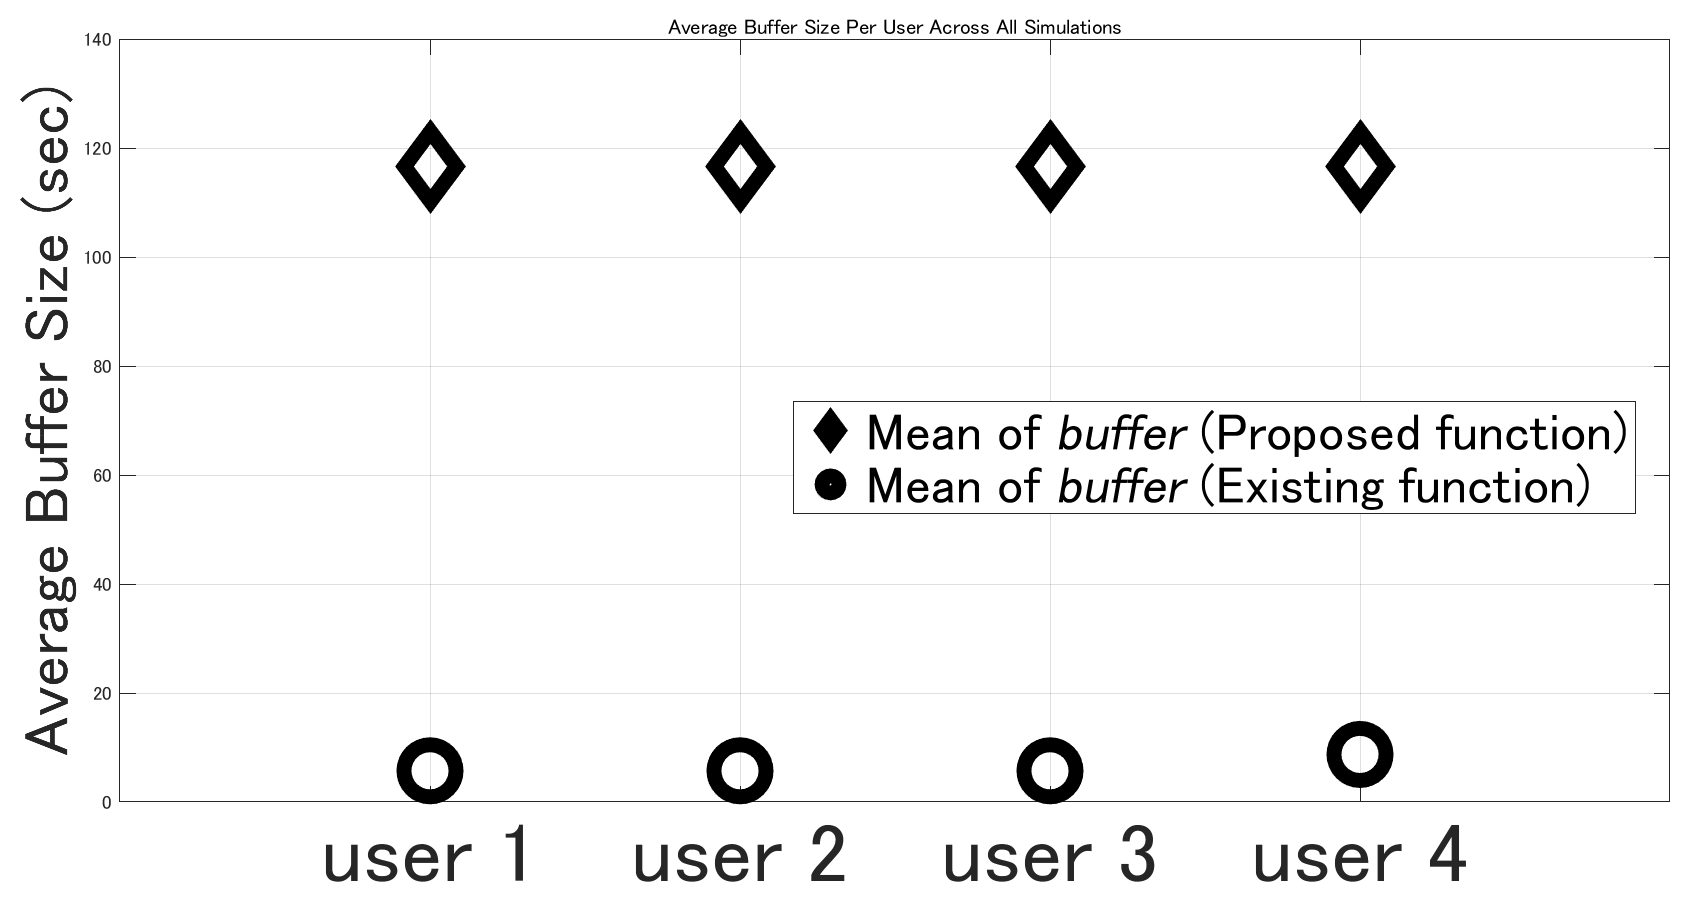
\includegraphics[scale=0.45]{hiritu_buffer.eps}
  \bicaption{平均貯蓄バッファ量の比較}%
            {Comparison of Average Savings Buffers}
    \label{fig:hiritu}
\end{figure}

図\ref{fig:hiritu}よりどのユーザにおいても,非協力ゲームレート制御\cite{kison}の利得関数\ref{eq:syousai}によって貯蓄されるバッファ量より,提案利得関数\ref{eq:proposed}によって貯蓄されるバッファ量の方が多いことが分かる.

これにより,提案する改良法は,非協力ゲームレート制御\cite{kison}よりバッファ枯渇による動画の再生中断が起こりにくいと言える.
\chapter{考察}
この章では,本研究の結果と.net Winter work shop 2024での議論を踏まえて,今後の展開について考察する.

提案された利得関数は,他ユーザの帯域利用状況を考慮して,利己的な高レート要求のユーザに対するペナルティを大きくする設計となっている.この利得関数の効果は,図\ref{fig:teianritoku}を見ると,ユーザ1が6Mbpsを要求し,ユーザ2が1Mbpsを要求した場合の利得変化に大きくに表れている.既存研究\cite{kison}\cite{motomoto}による図\ref{fig:kisonritoku}では,ユーザ1が6Mbpsを要求し,ユーザ2が1Mbpsを要求した場合ユーザ1の利得が-4.5であったのに対し,提案手法では-57.0という極端に低い値をとった.この52.5の利得低下は,提案手法が利己的なユーザにペナルティを課す仕組みを反映している.また,提案手法の特徴として,ユーザごとに異なるペナルティを課す点もある.利己的なユーザにペナルティを課す一方,リンクを共有している他ユーザが帯域に影響を与えないビデオビットレート要求の場合,そのユーザには利得低下のペナルティは与えず利得を保つことが保証される.既存研究\cite{kison}\cite{motomoto}では,利己的なユーザだけでなくリンクを共有する他ユーザにもペナルティを与える.これは表\ref{tb:ritoku1}を見れば明らかである.ユーザ1が6Mbpsを要求した場合,ユーザ1のみならずユーザ2も利得が減少する.しかし,提案利得関数ではユーザ2は利得が低下しない.それは表\ref{tab:teianritoku}を見れば明らかである.以下に表\ref{tab:teianritoku}を示す.
\begin{table}[h]
    \centering
    \bicaption{提案利得関数\ref{eq:f_buffi}の利得表}
                {Gain table for the proposed gain function\ref{eq:f_buffi}}
    \scalebox{0.7}{
    \begin{tabular}{|c|c|c|c|c|c|c|}
        \hline
        \diagbox{user1}{user2} & 1 & 2 & 3 & 4 & 5 & 6 \\ \hline
        1 & (0.5, 0.5) & (0.62, -1.0) & (0.67, -6.0) & (0.69, -16.0) & (0.7, -32.5) & (0.71, -57.0) \\ \hline
        2 & (-1.0, 0.62) & (0.0, 0.0) & (0.33, -2.62) & (0.5, -8.0) & (0.6, -16.88) & (0.67, -30.0) \\ \hline
        3 & (-6.0, 0.67) & (-2.62, 0.33) & (-1.5, -1.5) & (-0.94, -5.33) & (-0.6, -11.67) & (-0.37, -21.0) \\ \hline
        4 & (-16.0, 0.69) & (-8.0, 0.5) & (-5.33, -0.94) & (-4.0, -4.0) & (-3.2, -9.06) & (-2.67, -16.5) \\ \hline
        5 & (-32.5, 0.7) & (-16.88, 0.6) & (-11.67, -0.6) & (-9.06, -3.2) & (-7.5, -7.5) & (-6.46, -13.8) \\ \hline
        6 & (-57.0, 0.71) & (-30.0, 0.67) & (-21.0, -0.37) & (-16.5, -2.67) & (-13.8, -6.46) & (-12.0, -12.0) \\ \hline
    \end{tabular}
    \label{tab:teianritoku}
    }
\end{table}
これは既存研究\cite{kison}\cite{motomoto}の利得関数\ref{eq:f_{buffer}}では,バッファ変動量に基づいたシステム的なペナルティが設定されており,データ消費と貯蓄のバランスを重視している.一方で,提案利得関数\ref{eq:f_buffi}では,他ユーザとの比較を重視したペナルティ設計が行われており,この変更によりユーザの利得が相対的に評価されるようになった.この結果,帯域に影響を与えない低ビデオビットレート要求ユーザの利得が保たれ,高ビデオビットレート要求の利己的なユーザがより大きなペナルティを受ける仕組みが実現している.このように利得を制限することで,帯域に影響を与える高ビデオビットレートが最適レートとして導出されることを防ぐ.本研究では,ゲーム理論を用いてナッシュ均衡を導出することで,最適レートを導出している.ナッシュ均衡は各ユーザの利得の組み合わせがこれ以上大きくならないときのレートの組み合わせが選ばれる.そのため,利得を制限することで,そのレートの組み合わせが最適レートとして導出されないようにしている
しかし,利得が過剰に低下することで,ビデオビットレートも小さくなり,帯域利用の効率性やQoEの低下につながる可能性があるため,ペナルティのバランス調整が今後の課題となる.また,利得の下がり方がQoEにどのように影響するかについては,現状で明確な評価は行われていない.利得制限を反映させた初期段階であり,次のステップとして利得関数を基にしたレート制御を実現し,その上でQoE評価を行う必要がある.また,現時点ではユーザ数の増減に伴う利得の変化の解析が十分に検討されていない.ユーザ数が減少することで,一人当たりの帯域幅が増加し,高レート要求が選択されやすくなる一方,ユーザ数が増加すると,提案手法が帯域逼迫時にどのような挙動を示すかについての詳細な分析が必要である.

ゲーム理論を活用する意義についても議論があった.本研究ではゲーム理論を用いることで,利己的なユーザ間の相互作用をモデル化し,ナッシュ均衡解を導出している.単なる最適化やユーザの数で帯域を均等に割る手法では,ユーザ間の相互作用を考慮できないため,帯域幅の効率的な利用や公平性を担保することが難しい.本研究では,現時点でユーザ毎の特徴を考慮していない.Wangら\cite{C.Wang}は,ユーザの行動などの特性が動画視聴のQoEに影響を及ぼすことを示唆している.例えば,ラジオ感覚で動画を流し見するユーザや動画を高画質で視聴するユーザもいる.このようなユーザはそれぞれ要求するビデオビットレートが異なるため,帯域をユーザ数で等分する手法では,ユーザの公平性が担保されない.ゲーム理論を用いることで,非協力的なユーザが存在する状況下でも安定的な最適レートを導出することが可能である.しかし,現在ユーザ毎の行動特性を考慮していないため,今後特性を取り入れた関数の作成が検討される.また現状では,ユーザ全体の利得合計が既存手法に比べて低下する傾向が見られる.この点について,QoEを向上させるための調整が必要である.利得が極端に低い値を取る場合,帯域幅に余裕があるにも関わらず低レートしか選択されない状況が生じる可能性があるため,これを防ぐためのさらなる改良が求められる.

今後の研究では,以下の方向性を重点的に進める必要がある.まず,視聴動画の種類や画質要求の違いなど,ユーザ特性を利得関数に組み込むことで,より個別化されたレート制御を実現することが求められる.また,現在は利得の変化に基づいた評価が中心であるが,最終的にはQoEの向上を実証する必要がある.具体的には,提案手法を用いた場合のユーザ満足度の向上を定量的に評価する必要がある.さらに,現行のペナルティ項の構造を再評価し,よりシンプルかつ効果的な設計を模索する必要がある.加えて,現状では$2\sim4$人のユーザを対象としているが,多人数ユーザ環境における提案手法の有効性を検証することも重要である.

以上の方向性に基づき,提案手法の改善と実用性の向上を図ることで,QoE向上を目指したレート制御法の考案を今後検討する.
\chapter{結論}
本研究では,ユーザの利己的なビデオビットレート要求が他ユーザの使用帯域に与える影響を考慮した利得関数への改良を提案した.この利得関数により,帯域に影響を与えない低ビットレートを要求するユーザに対して過渡な制限を課すことなく,各ユーザの影響度に応じた効率的な帯域割り当ての実現性を示した.また,既存研究\cite{kison}と比較し,貯蓄されるバッファ量が多いため,動画の再生停止が起きにくいことが示された.
しかし,本研究には以下の課題が残されている.第一に,本研究では利得関数の利得制限の改良を行ったのみである為,実際の動画再生中における持続的かつ動的なレート制御が十分に実現されていない.特に,帯域の急激な変動やリンクへの複数ユーザの離脱や加入が発生した場合の影響を,時間的な変化に沿って解析することが求められる.
第二に,提案手法の評価ではバッファ量や利得を中心とした分析を行ったが,ユーザのQoEについての評価まで解析できていない課題がある.既存研究\cite{kison}では導出された最適レートを基にユーザごとの平均QoEを算出し評価しているため,QoEに関する比較分析が不十分である.
今後は,提案した利得関数の様々の条件でのQoE解析や関数自体の改善を検討する.
\input{chapter7}

\chapter*{謝辞}
\addcontentsline{toc}{chapter}{謝辞}
本論文を執筆するにあたり,1年間ご指導いただいた上岡先生に感謝いたします.
また,貴重なご意見を頂いた東京科学大学の宮田先生並びに山岡先生,大阪大学の黒川先生に感謝いたします.
そして,1年間,助言や議論をしてくれた先輩方や同期,そして山岡研究室の皆様にも感謝いたします.

\chapter*{付録}
以下に,.net Winter Workshop 2024で使用した発表資料を付録として添付する.

\begin{figure}[th]
  \centering
  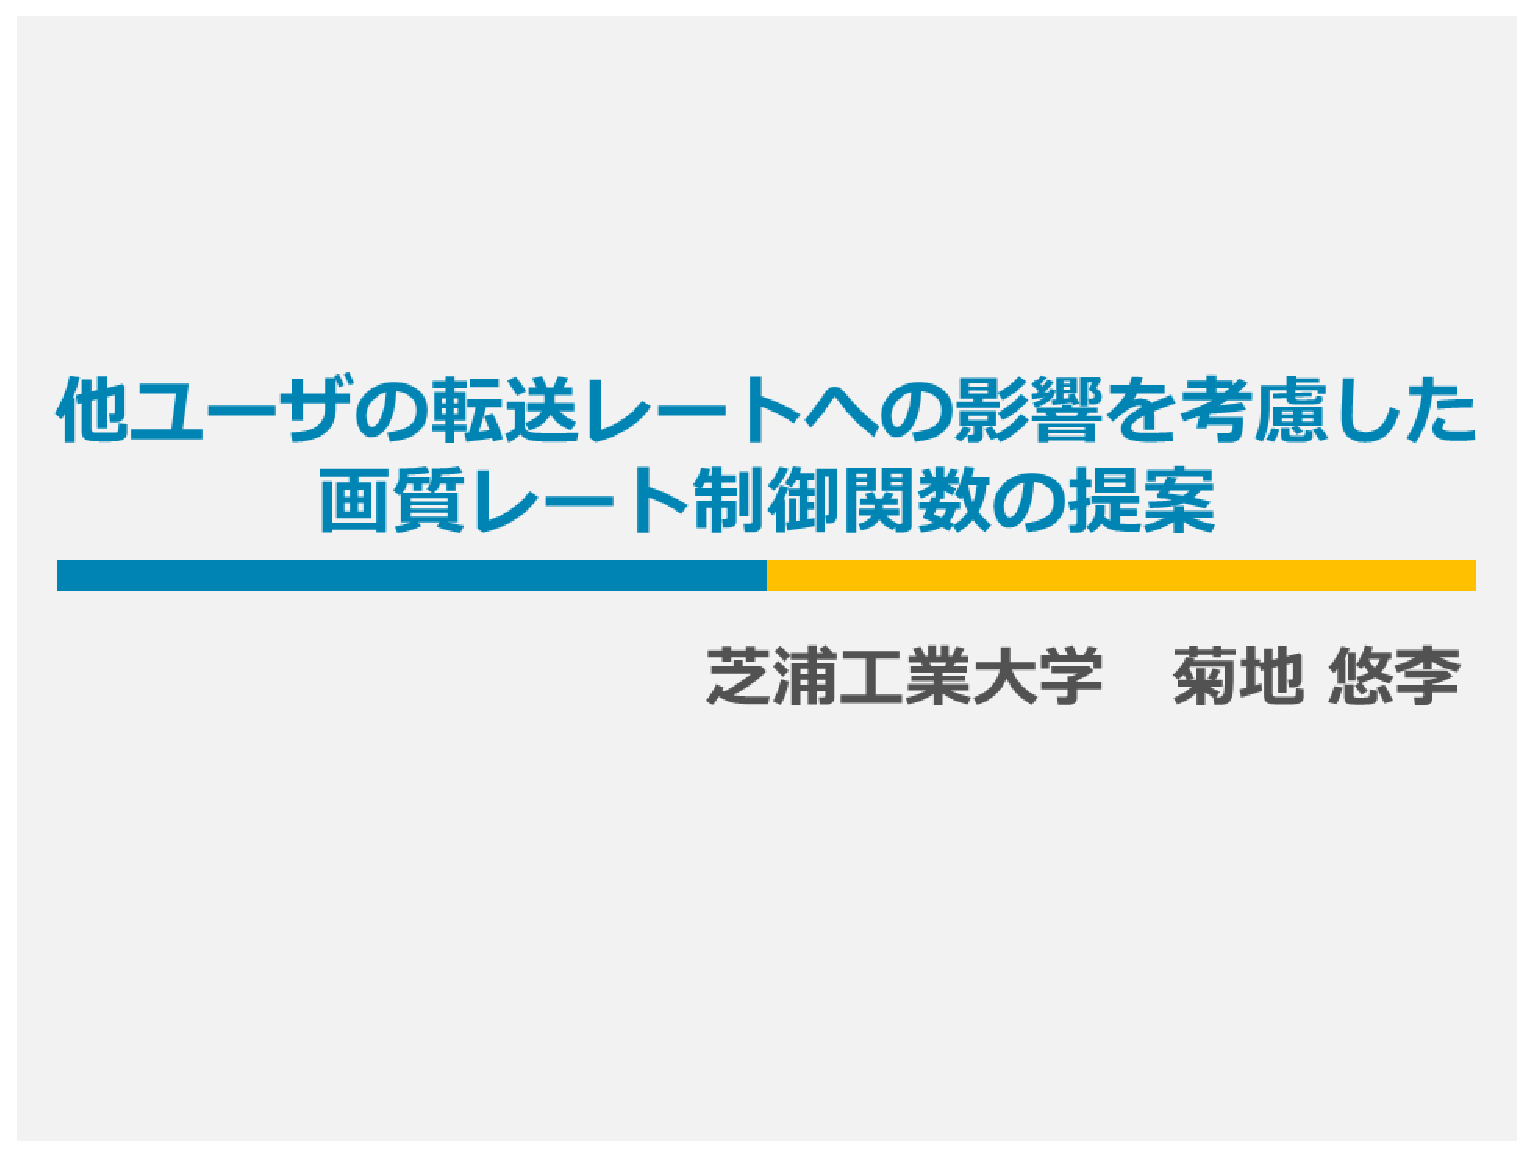
\includegraphics[scale=0.45]{1.eps}
\end{figure}

\begin{figure}[b]
  \centering
  \includegraphics[scale=0.45]{2.eps}
\end{figure}

\begin{figure}[tp]
  \centering
  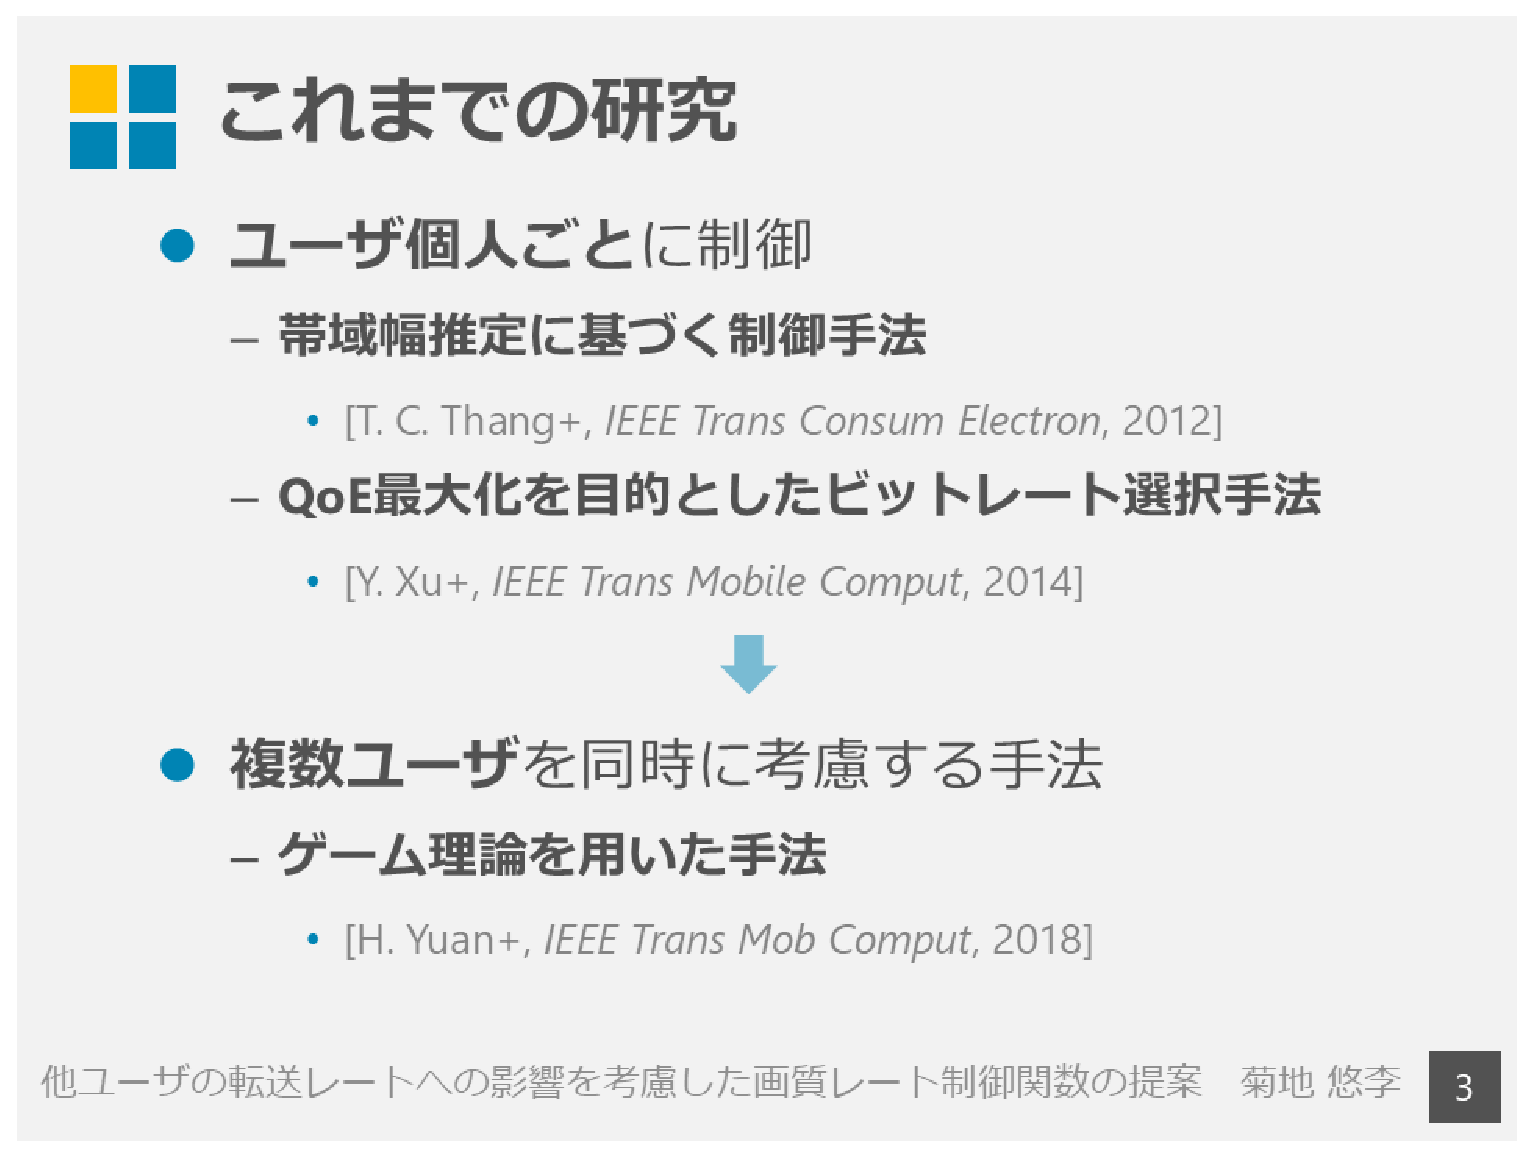
\includegraphics[scale=0.45]{3.eps}
\end{figure}

\begin{figure}[tb]
  \centering
  \includegraphics[scale=0.45]{4.eps}
\end{figure}

\begin{figure}[tp]
  \centering
  \includegraphics[scale=0.45]{5.eps}
\end{figure}

\begin{figure}[tb]
  \centering
  \includegraphics[scale=0.45]{6.eps}
\end{figure}

\begin{figure}[tp]
  \centering
  \includegraphics[scale=0.45]{7.eps}
\end{figure}

\begin{figure}[tb]
  \centering
  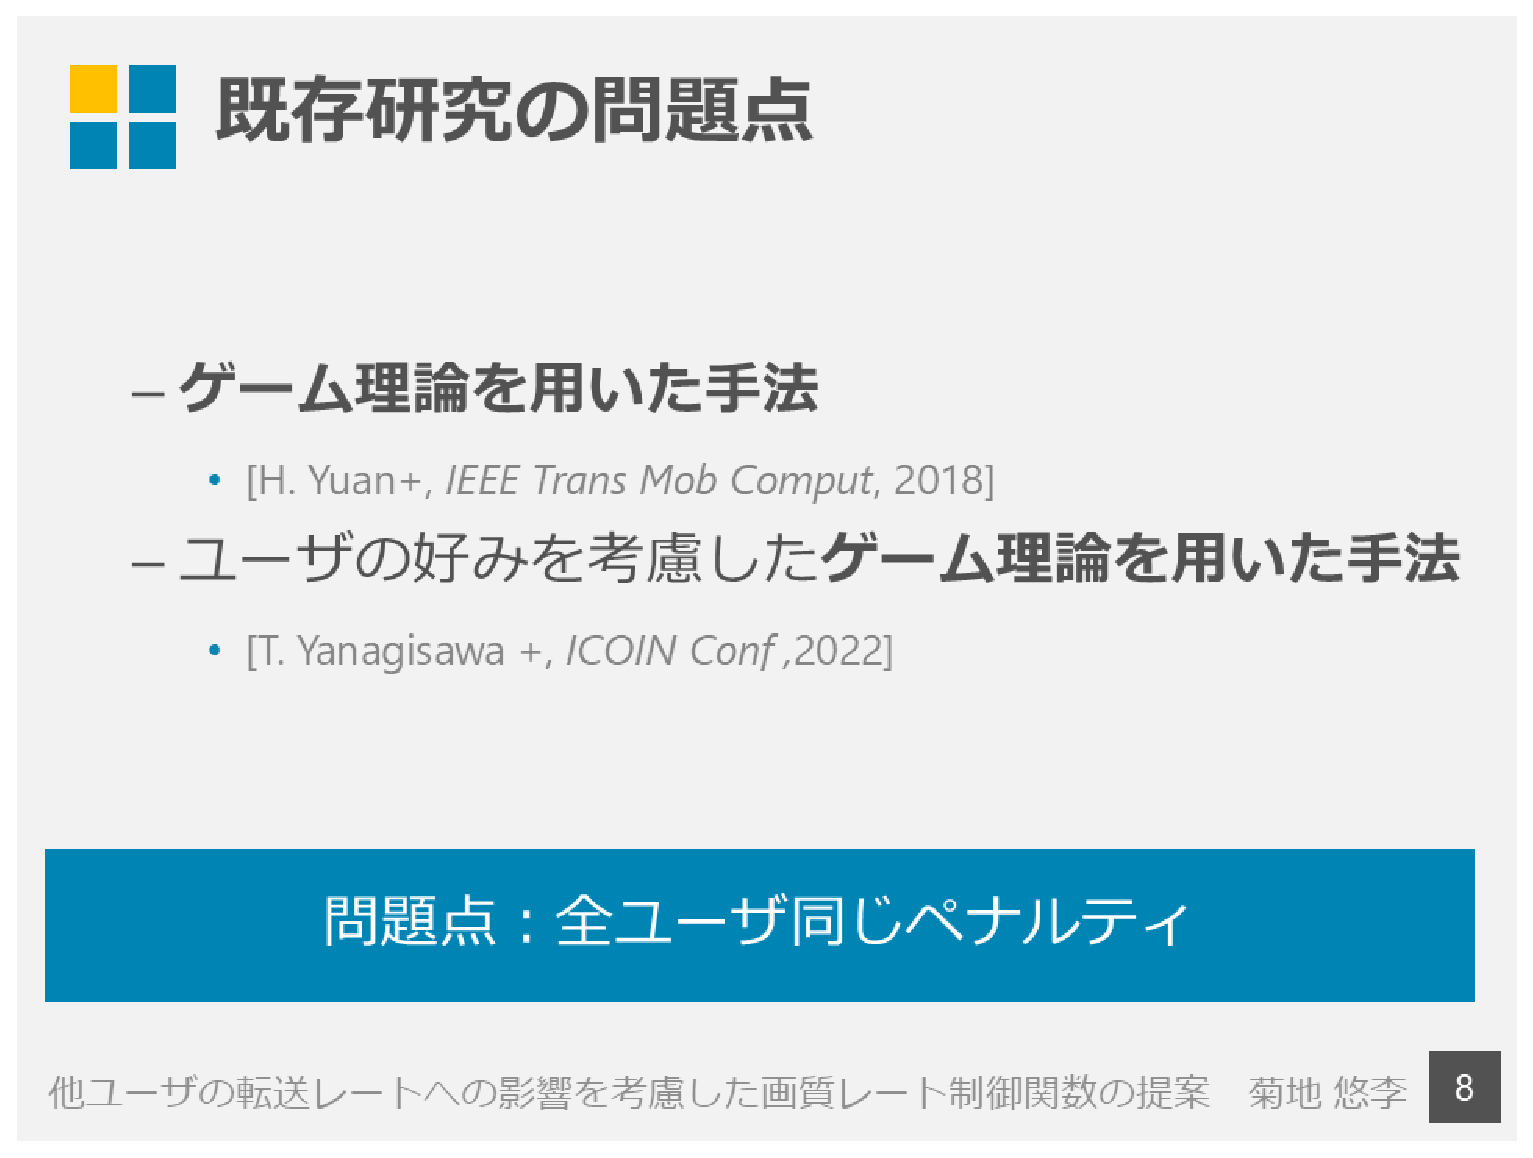
\includegraphics[scale=0.45]{8.eps}
\end{figure}

\begin{figure}[tp]
  \centering
  \includegraphics[scale=0.45]{9.eps}
\end{figure}

\begin{figure}[tb]
  \centering
  \includegraphics[scale=0.45]{10.eps}
\end{figure}

\begin{figure}[tp]
  \centering
  \includegraphics[scale=0.45]{11.eps}
\end{figure}

\begin{figure}[tb]
  \centering
  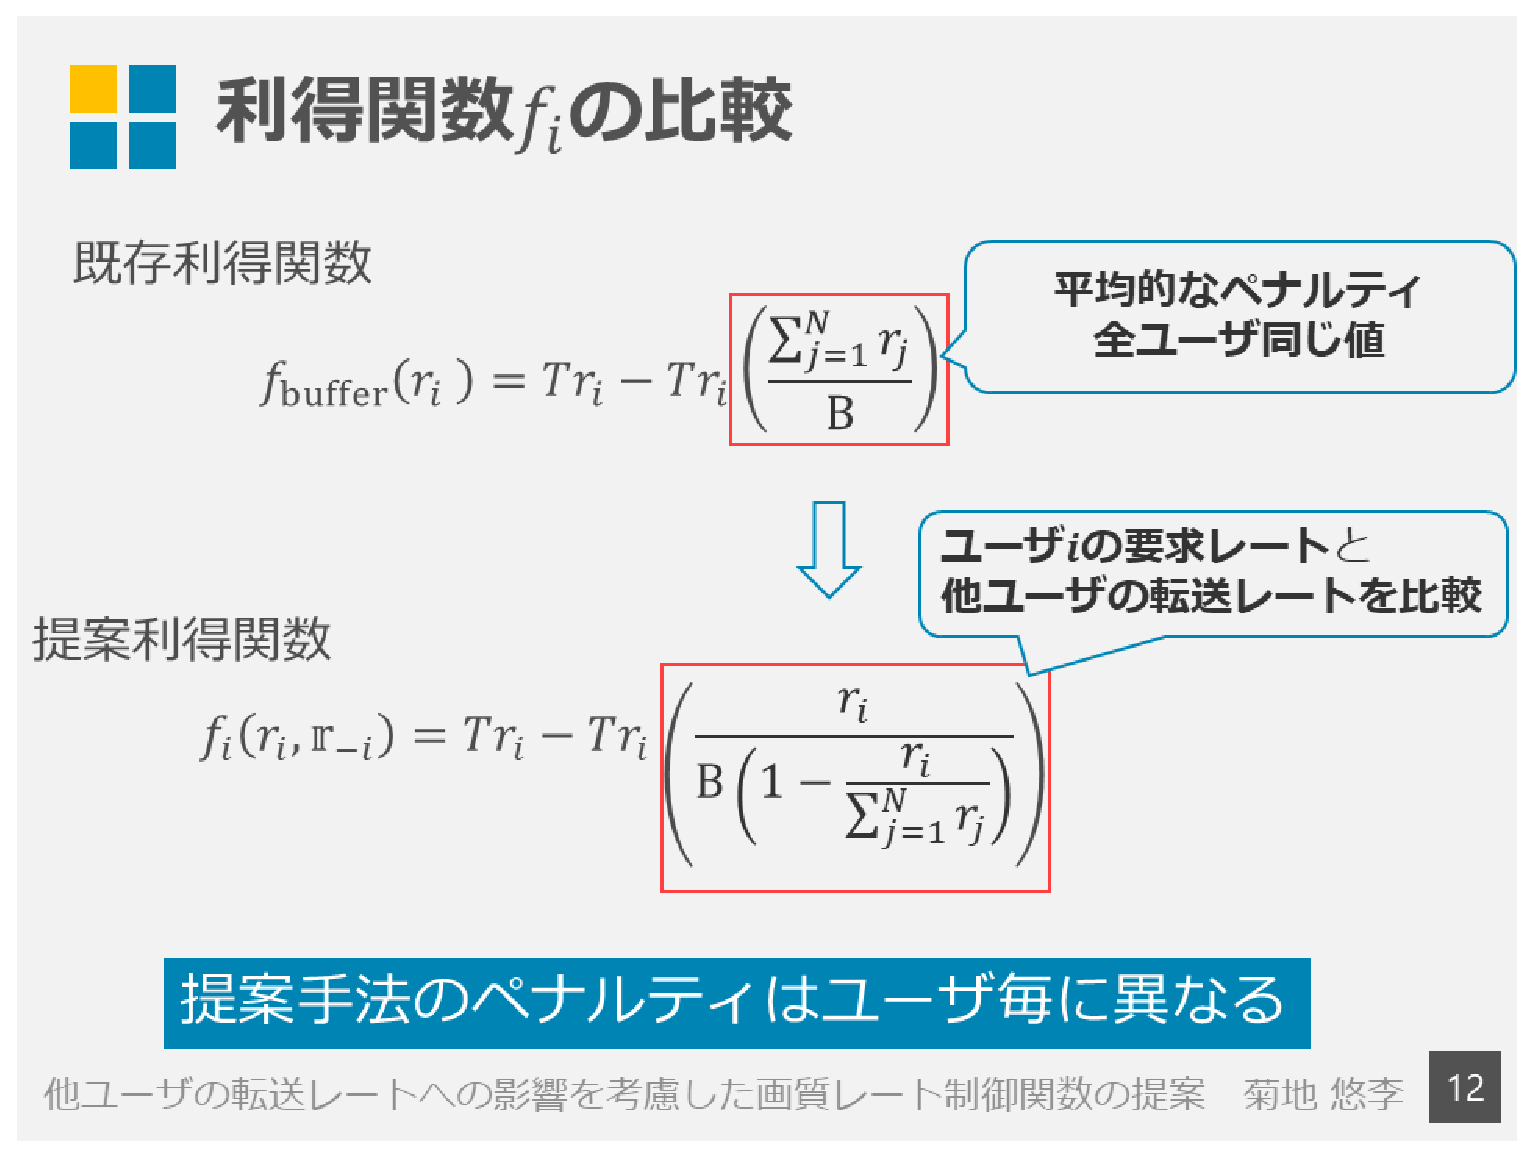
\includegraphics[scale=0.45]{12.eps}
\end{figure}

\begin{figure}[tp]
  \centering
  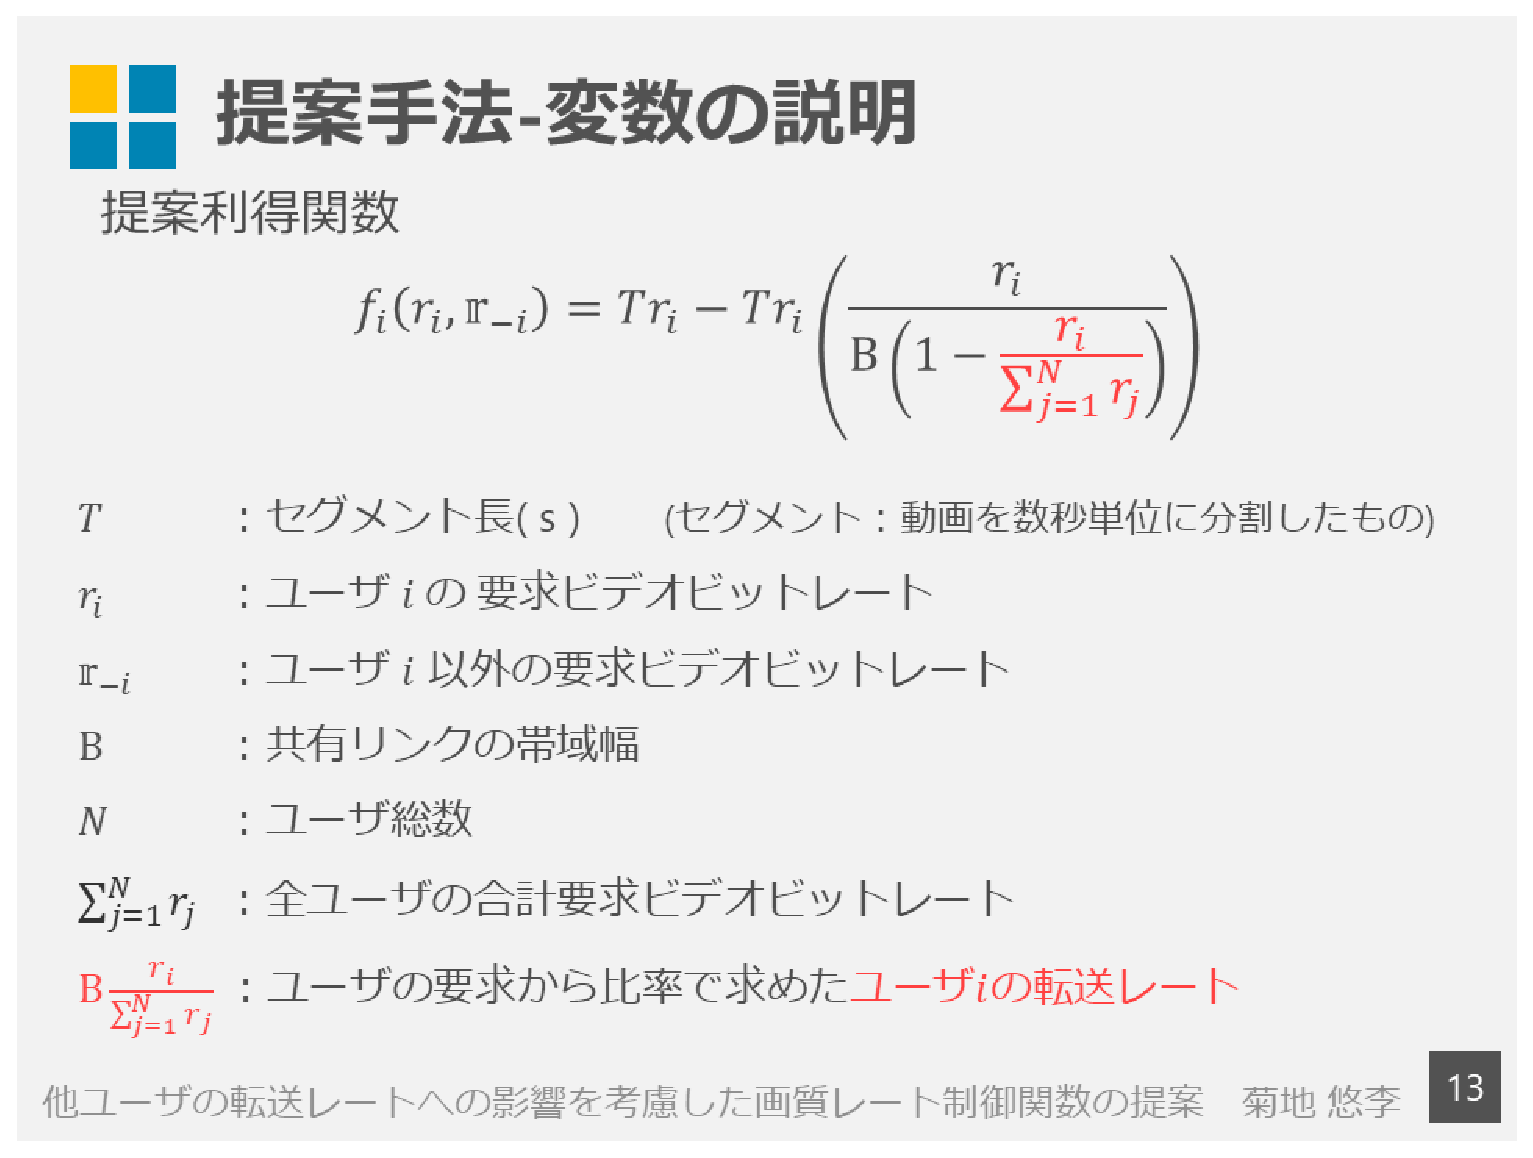
\includegraphics[scale=0.45]{13.eps}
\end{figure}

\begin{figure}[tb]
  \centering
  \includegraphics[scale=0.45]{14.eps}
\end{figure}

\begin{figure}[tp]
  \centering
  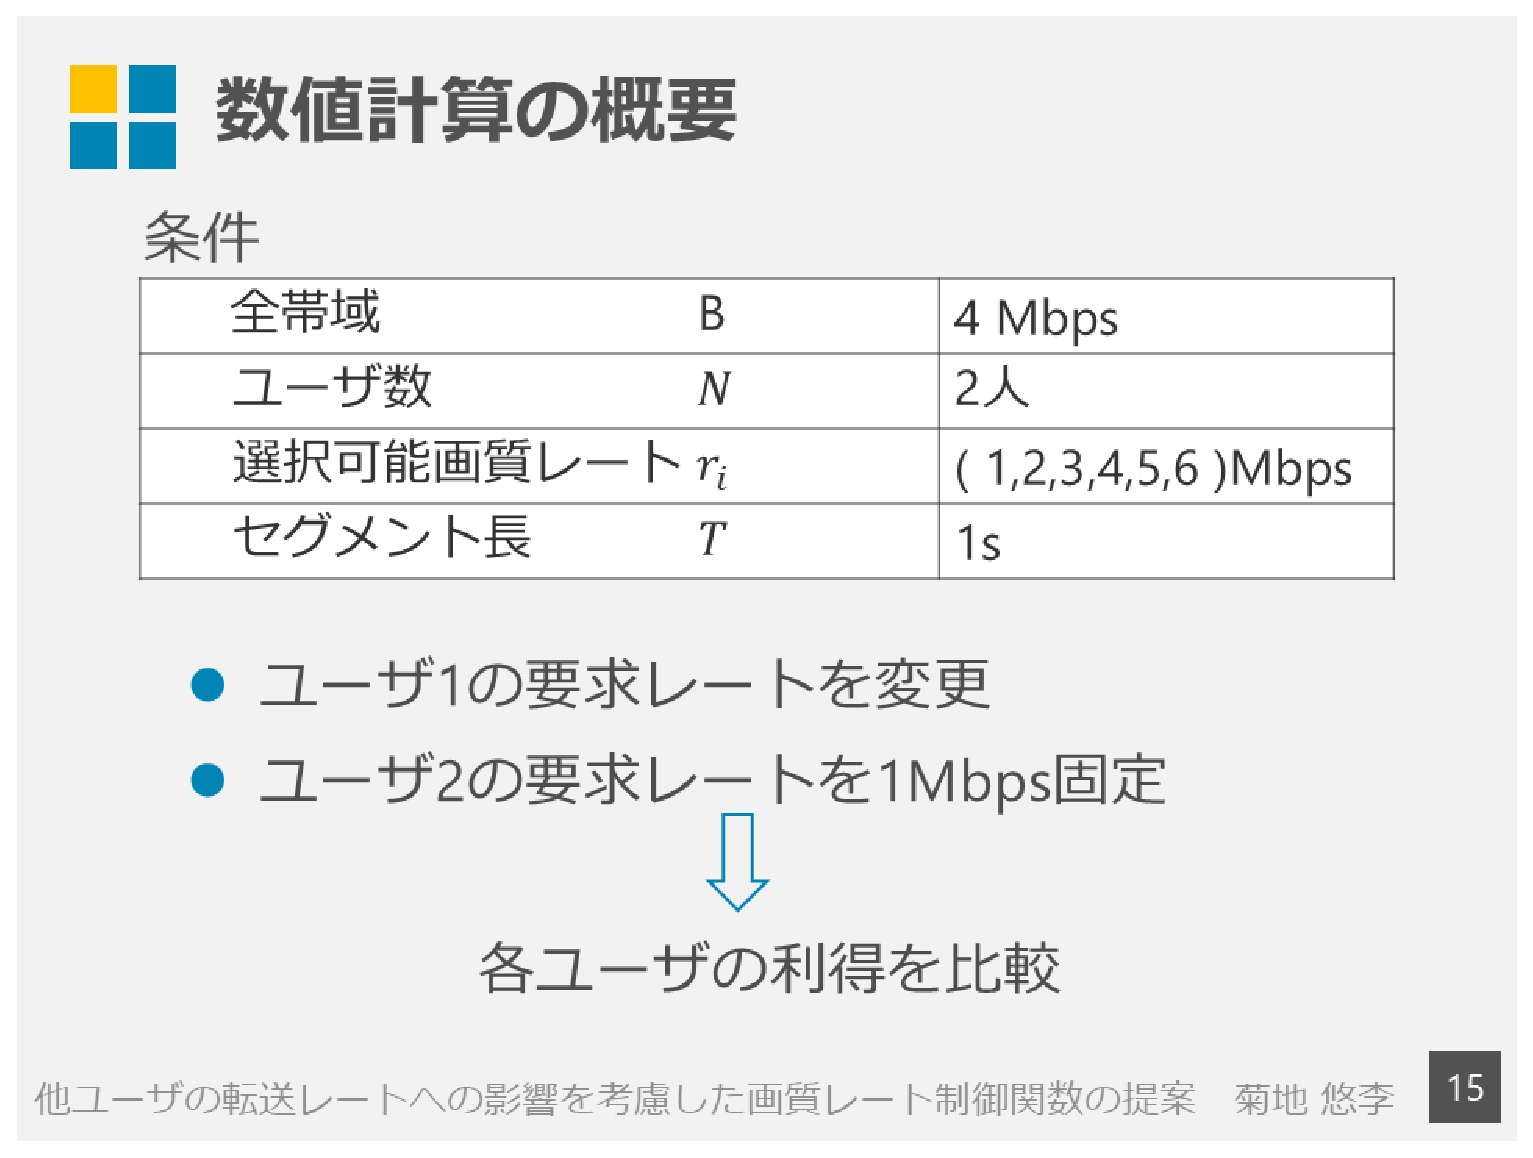
\includegraphics[scale=0.45]{15.eps}
\end{figure}

\begin{figure}[tb]
  \centering
  \includegraphics[scale=0.45]{16.eps}
\end{figure}

\begin{figure}[tp]
  \centering
  \includegraphics[scale=0.45]{17.eps}
\end{figure}

\begin{figure}[tb]
  \centering
  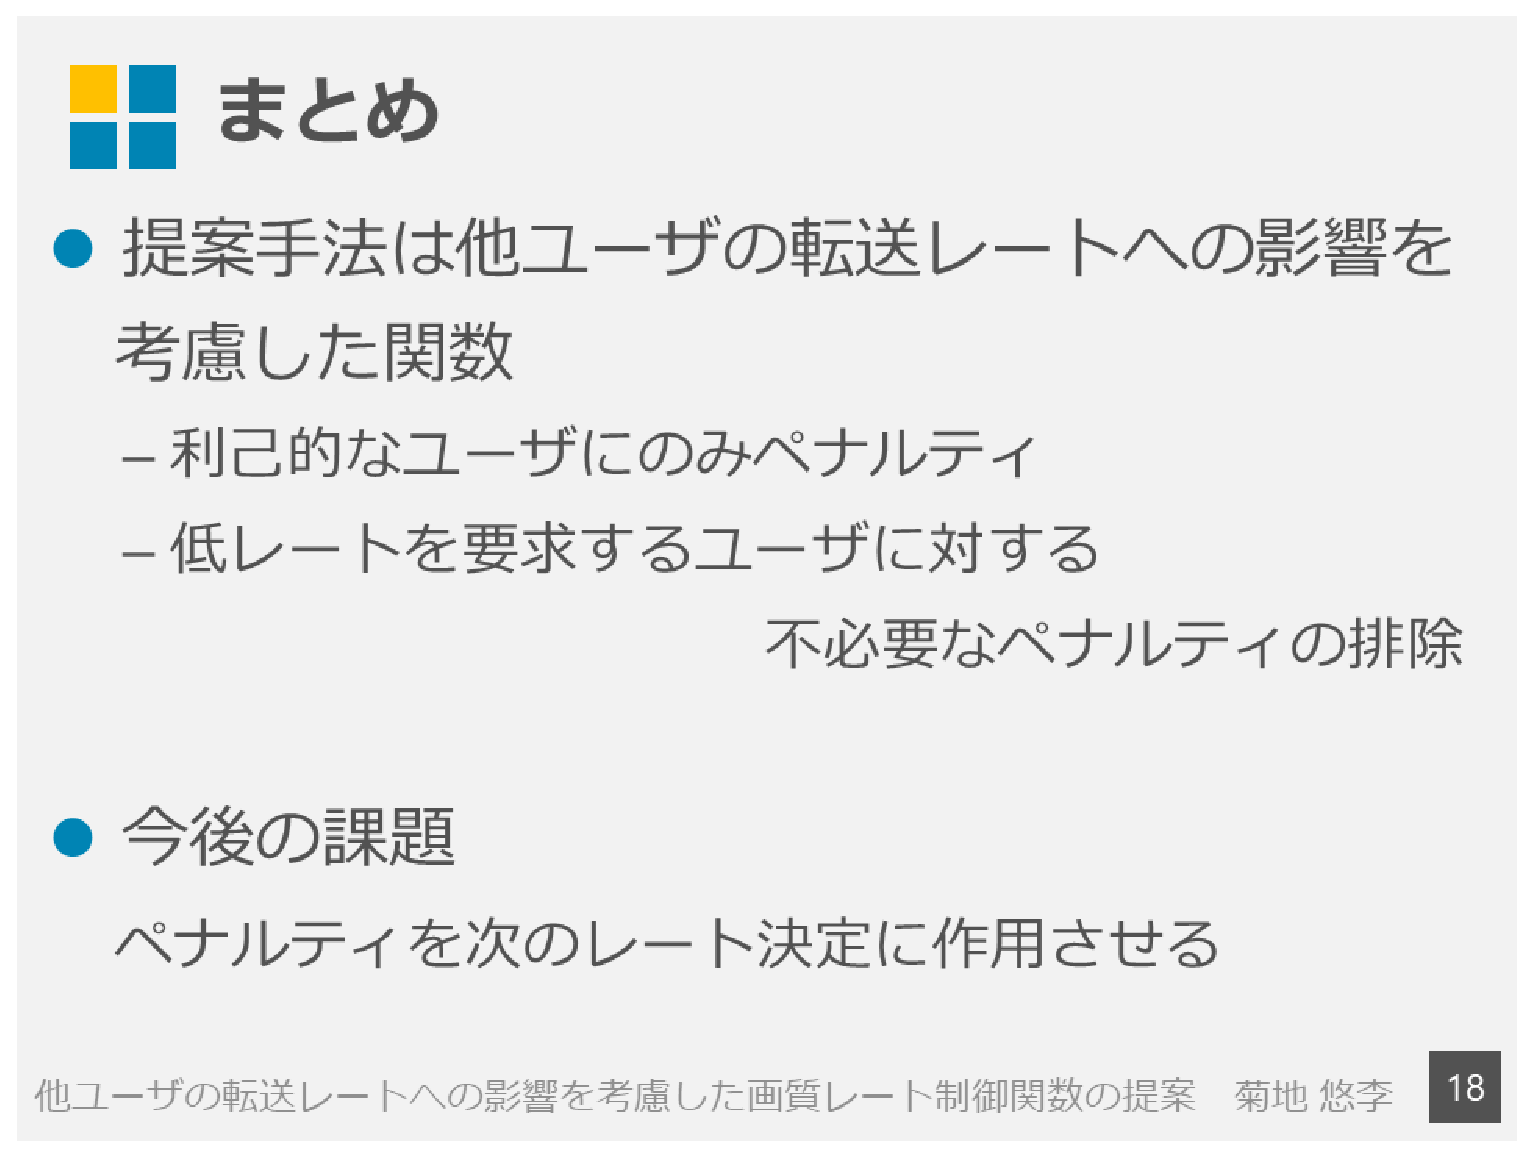
\includegraphics[scale=0.45]{18.eps}
\end{figure}



%%%%%%%%%%%%%%%%%%%%%%%%%%%%%%%%%%%%%%%%%%%%%%%%%%%%%%%%%%%%%%%%
\begin{thebibliography}{99}
    \bibitem{kison} T. Yanagisawa, "DASH rate control using game theory to consider user video preference," 
    Proc. of the 2022 International Conference on Information Networking (ICOIN), pp. 113--118, Jan. 2022, doi:10.1109/ICOIN53446.2022.9687211.

    \bibitem{motomoto} H. Yuan, {\it et al.}, "Non-Cooperative Game Theory Based Rate Adaptation for Dynamic Video Streaming over HTTP," 
    IEEE Transactions on Mobile Computing, Vol. 17, No. 10, pp. 2334--2348, Oct. 2018.

    \bibitem{okada2011} 岡田章, 『ゲーム理論 新版』, 有斐閣, 2011.

    \bibitem{C.Wang} C. Wang, A. Rizk, and M. Zink, "SQUAD: a spectrum-based quality adaptation for dynamic adaptive streaming over HTTP," in \textit{Proceedings of the 7th International Conference on Multimedia Systems (MMSys '16)}, Klagenfurt, Austria, Association for Computing Machinery, New York, NY, USA, 2016, doi: 10.1145/2910017.2910593.

    \bibitem{Thang} T. C. Thang, Q.-D. Ho, J. W. Kang, and A. T. Pham, "Adaptive streaming of audiovisual content using MPEG DASH," 
    IEEE Transactions on Consumer Electronics, vol. 58, no. 1, pp. 78--85, Feb. 2012, doi: 10.1109/TCE.2012.6170058.

    \bibitem{Mao} H. Mao, R. Netravali, and M. Alizadeh, "Neural Adaptive Video Streaming with Pensieve," in \textit{Proceedings of the Conference of the ACM Special Interest Group on Data Communication (SIGCOMM '17)}, pp. 197--210, Aug. 2017, doi: 10.1145/3098822.3098843.

    \bibitem{Xu} Y. Xu, Y. Zhou, and D.-M. Chiu, "Analytical QoE Models for Bit-Rate Switching in Dynamic Adaptive Streaming Systems," \textit{IEEE Transactions on Mobile Computing}, vol. 13, no. 12, pp. 2734--2748, Dec. 2014, doi: 10.1109/TMC.2014.2307323.

    \bibitem{johari} R. Johari and J. N. Tsitsiklis, "A Game Theoretic View of Efficiency Loss in Resource Allocation," in \textit{Advances in Control, Communication Networks, and Transportation Systems: In Honor of Pravin Varaiya}, E. H. Abed, Ed., Boston, MA: Birkhäuser Boston, 2005, pp. 203--223, doi: 10.1007/0-8176-4409-10-12.

    \bibitem{cisco2018} Cisco Systems, "Cisco Annual Internet Report (2018–2023)," Cisco White Paper, pp. 1--147, 2020.

    \bibitem{Y.Huang} Y. Huang, W. Zhou, and Y. Du, "A study on the user behavior-based QoE evaluation method for HTTP mobile streaming," in \textit{Proceedings of the 9th International Conference on Broadband and Wireless Computing, Communication and Applications (BWCCA '14)}, Guangdong, China, 2014, pp. 47–51, doi: 10.1109/BWCCA.2014.14.
\end{thebibliography}


\end{document}








